\documentclass[twoside,twocolumn]{article}

% for vector diagrams.
\usepackage{tikz}
\usetikzlibrary{arrows,quotes,angles}
\usetikzlibrary{}

\usepackage{amsmath} % for \eqref
\usepackage{graphicx} % for including images.

\usepackage{blindtext} % Package to generate dummy text throughout this template

\usepackage[sc]{mathpazo} % Use the Palatino font
\usepackage[T1]{fontenc} % Use 8-bit encoding that has 256 glyphs
\linespread{1.05} % Line spacing - Palatino needs more space between lines
\usepackage{microtype} % Slightly tweak font spacing for aesthetics

% textcomp package inclusion prevents the following warning:
% Font shape `OMS/pplx/m/n' undefined using `OMS/cmsy/m/n' instead for symbol `textasteriskcentered'
\usepackage{textcomp}

\usepackage[english]{babel} % Language hyphenation and typographical rules

\usepackage[hmarginratio=1:1,top=32mm,columnsep=20pt]{geometry} % Document margins
\usepackage[hang, small,labelfont=bf,up,textfont=it,up]{caption} % Custom captions under/above floats in tables or figures
\usepackage{booktabs} % Horizontal rules in tables

\usepackage{lettrine} % The lettrine is the first enlarged letter at the beginning of the text

\usepackage{enumitem} % Customized lists
\setlist[itemize]{noitemsep} % Make itemize lists more compact

\usepackage{abstract} % Allows abstract customization
\renewcommand{\abstractnamefont}{\normalfont\bfseries} % Set the "Abstract" text to bold
\renewcommand{\abstracttextfont}{\normalfont\small\itshape} % Set the abstract itself to small italic text

\usepackage{titlesec} % Allows customization of titles
\renewcommand\thesection{\Roman{section}} % Roman numerals for the sections
\renewcommand\thesubsection{\roman{subsection}} % roman numerals for subsections
\titleformat{\section}[block]{\large\scshape\centering}{\thesection.}{1em}{} % Change the look of the section titles
\titleformat{\subsection}[block]{\large}{\thesubsection.}{1em}{} % Change the look of the section titles

%\usepackage{fancyhdr} % Headers and footers
%\pagestyle{fancy} % All pages have headers and footers
%\fancyhead{} % Blank out the default header
%\fancyfoot{} % Blank out the default footer
%\fancyhead[C]{Running title $\bullet$ May 2016 $\bullet$ Vol. XXI, No. 1} % Custom header text
%\fancyfoot[RO,LE]{\thepage} % Custom footer text

\usepackage{titling} % Customizing the title section

\usepackage{hyperref} % For hyperlinks in the PDF

\setlength{\droptitle}{-4\baselineskip} % Move the title up

\pretitle{\begin{center}\Huge\bfseries} % Article title formatting
\posttitle{\end{center}} % Article title closing formatting
\title{[DRAFT] Towards a Better Understanding of Lift and Drag: Deflection Theory} % Article title

\author{
%\textsc{Robert Lee} \\[1ex] % Your name
%\normalsize University of California \\ % Your institution
%\normalsize \href{mailto:robhlee32@gmail.com}{robhlee32@gmail.com} % Your email address
%\and % Uncomment if 2 authors are required, duplicate these 4 lines if more
%\textsc{Jane Smith}\thanks{Corresponding author} \\[1ex] % Second author's name
%\normalsize University of Utah \\ % Second author's institution
%\normalsize \href{mailto:jane@smith.com}{jane@smith.com} % Second author's email address
}

%\date{\today} % Leave empty to omit a date
\date{} % Leave empty to omit a date

\renewcommand{\maketitlehookd}{
\begin{abstract}
\noindent
"Deflection Theory" is an application of Newton's Third Law to the interaction between airfoils and freestream flow that physically couples lift and drag, even in incompressible and inviscid flow.
The current consensus is that airfoils in incompressible and inviscid flow cannot produce drag.
Deflection Theory introduces the concept of modeling the change in direction of the portion of the freestream that interacts with the airfoil.
NACA 0009 experimental data corroborate lift, drag, and lift-to-drag ratio predictions.
\end{abstract}

}


\begin{document}

% Print the title
\maketitle

% ARTICLE CONTENTS
\section{Introduction}
Current airfoil performance models for incompressible and inviscid flow predict lift without drag.
Conservation of energy dictates that airfoil forces cannot be parallel to freestream flow at the airfoil,
and this is the reason for d'Alembert's Paradox.
Aerodynamic forces in inviscid and incompressible potential flow are therefore normal to the flow direction at the airfoil
, and drag comes from this change in flow direction.
In the three-dimensional context, trailing wake vortex modeling tilts flow at the airfoil to cause "lift-induced drag".
However, no well-known direct relationship between lift and drag exists for the purely two-dimensional context.
Deflection Theory offers an explanation for two-dimensional "lift-coupled drag".

Thin Airfoil Theory and the Vortex Panel Method assume a fixed freestream flow, independent of any forces exerted on the airfoil.
By the conservation of momentum, freestream flow downstream of the airfoil should be deflected to oppose the resultant aerodynamic forces on the airfoil.
Dragless lift is a valid transient solution, but not a steady-state one.
Deflection Theory is able to predict drag as naturally as lift because the conservation of momentum is applied to the portion of freestream flow that interacts with the airfoil.

The common lift-producing spinning cylinder example clearly shows the deficiency of current lift and drag analysis methods.
Everyone would agree that generally speaking, an airfoil produces lift by "pushing down" air, and this could be said of any object that produces lift.
However, the traditional spinning cylinder solution has a flow field with velocity magnitudes and streamlines exactly symmetrical from fore and aft of the cylinder.
This clearly implies that just as much air is pulled up as it is pushed down. This clearly violates Newton's Third Law.


\section{Methods}

Newton's Third Law dictates that air must be deflected in opposition to airfoil lift force.
It will be shown that such deflection also causes drag, which means drag is coupled with lift.
Lift without drag therefore voilates Newton's Third Law.

\begin{figure}
\begin{tikzpicture}
    % horizontal dotted line.
    \draw (-3, 0) coordinate (upstream) node {};
    \draw (3, 0) coordinate (end) node {};
    \draw[dotted] (upstream) -- (end);
    % Region labels.
    \node[draw] at (-2.5, 1.5) {Upstream};
    \node[draw] at (-0.25, 1.5) {At airfoil};
    \node[draw] at (2.25, 1.5) {Downstream};
    % vertical dotted lines, separating regions.
    \draw (-1.5, 2) coordinate (top1) node {};
    \draw (-1.5, -2) coordinate (bottom1) node {};
    \draw[dotted] (top1) -- (bottom1);
    \draw (1, 2) coordinate (top2) node {};
    \draw (1, -2) coordinate (bottom2) node {};
    \draw[dotted] (top2) -- (bottom2);
    % upstream vector.
    \draw (-3, 0.25) coordinate (upstream label) node {$V_\infty$};
    \draw (-2, 0) coordinate (upstream tip) node {};
    \draw[->, >=latex] (upstream) -- (upstream tip);
    % airfoil vector.
    \draw (-1, 0) coordinate (airfoil root) node {};
    \draw (-0.06031, -0.34202) coordinate (airfoil tip) node {};
    \draw[->, >=latex] (airfoil root) -- (airfoil tip);
    \draw pic["", draw=orange, <->, angle eccentricity=1.2, angle radius=0.75cm]
        {angle=airfoil tip--airfoil root--end};
    \draw (0.25, -0.1) coordinate (airfoil angle label) node {$\phi/2$};
    % downstream vector.
    \draw (1.4, 0) coordinate (downstream root) node {};
    \draw (2.16604, -0.64279) coordinate (downstream tip) node {};
    \draw[->, >=latex] (downstream root) -- (downstream tip);
    \draw pic["$\phi$", draw=orange, <->, angle eccentricity=1.2, angle radius=0.75cm]
        {angle=downstream tip--downstream root--end};
\end{tikzpicture}
    \caption{Vector illustration flow direction changes (angles exaggerated). Vector magnitudes remain the same.}
\end{figure}

Suppose the portion of the freestream flow that interacts with the airfoil has a mass flow rate of \(\dot{m}\) and a velocity \(V_\infty\).
If we take the average angle of deflection of the airflow to be \(\phi\), lift (\(L\)) and drag (\(D\)) can be calculated as:

\begin{equation}
\label{eq:lift}
    L = \dot{m} V_\infty sin(\phi)
\end{equation}

\begin{equation}
D = \dot{m} V_\infty (1 - cos(\phi))
\label{eq:drag}
\end{equation}

\begin{equation}
\frac{L}{D} = \frac{sin(\phi)}{1 - cos(\phi)}
\end{equation}

Since airfoils in incompressible and inviscid flow can not produce forces parallel to the flow at the airfoil, the relationship between the induced flow angle (\(\gamma\)) and the lift-to-drag ratio is:

\begin{equation}
\frac{L}{D} = \frac{cos(\gamma)}{sin(\gamma)}
\end{equation}

Equating the two expressions for lift-to-drag ratio:

\begin{equation}
\frac{sin(\phi)}{1 - cos(\phi)}
    = \frac{cos(\gamma)}{sin(\gamma)}
\end{equation}

Through trigometric identities:

\begin{equation}
    \gamma = \frac{\phi}{2}
\end{equation}

The airfoil "sees" the freestream tilted at an angle exactly half that of the full deflection angle downstream of the airfoil.

To relate \(C_N\) and the deflection angle \(\phi\):

\begin{equation}
\label{eq:force}
    F = \sqrt{L^2 + D^2}
\end{equation}

Where \(A_\infty\) is the mass flux area of the freestream that interacts with the airfoil:

\begin{equation}
\label{eq:mdot}
    \dot{m} = \rho A_\infty V_\infty
\end{equation}

Substituting \(\eqref{eq:lift}\), \(\eqref{eq:drag}\), and \(\eqref{eq:mdot}\) into \(\eqref{eq:force}\):

\begin{equation}
    F = \rho A_\infty V_\infty^2 \sqrt{2 - 2 cos(\phi)}
\end{equation}

Normalizing \(F\) to \(C_N\):

\begin{equation}
    C_N = \frac{A_\infty} {A_w} \sqrt{8 - 8 cos(\phi)}
\end{equation}

The ratio \(A_\infty / A_w\), where \(A_w\) is the reference area of the wing, is the final loose end of Deflection Theory. Unfortunately at present I do not have a physical way to estimate this parameter.
\(A_\infty / A_w\) may be constant, or dependent on the force exerted on the airfoil, or something else.
Presently the ratio is chosen arbitrarily as to reasonably match the experimental data to demonstrate Deflection Theory's potential.

We can utilize existing performance prediction methods such as Thin Airfoil Theory and Vortex Panel Method by simply taking their results as the normal force coefficient \(C_N\), instead of, as traditionally assumed, the lift coefficient \(C_L\). For simplicity, we will use Thin Airfoil Theory to obtain a relationship between angle of attack (\(\alpha\)) and \(C_N\):

\begin{equation}
    C_N = 2 \pi \alpha
\end{equation}

We must make the distinction between the aerodynamic angle of attack (\(\alpha\)) and the global angle of attack (\(\alpha_g\)):

\begin{equation}
    \alpha_g = \gamma + \alpha
\end{equation}

NACA 0009 airfoil data were chosen for comparison, because it is a thin and symmetric airfoil and has publicly available performance data. The minimum drag coefficient from experimental data was added to the Deflection Theory model to account for skin friction and baseline unsteady drag.


\section{Results}

Figures \ref{fig:cl}, \ref{fig:cd}, and \ref{fig:ld} demonstrate Deflection Theory's efficacy up until stall.

\graphicspath{{./}}

\begin{figure}[htb]
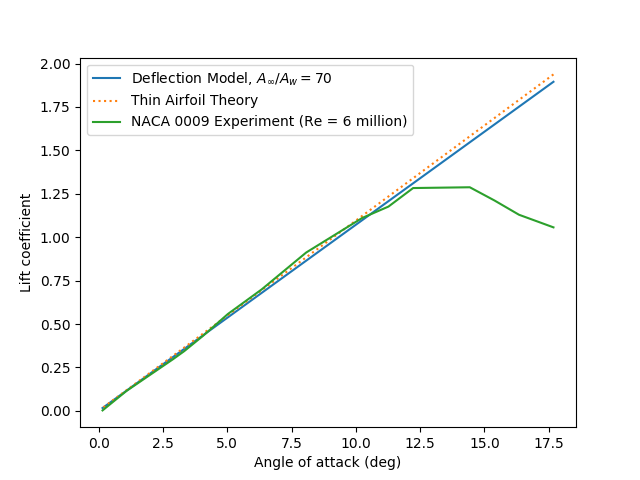
\includegraphics[totalheight=4.5cm]{cl}
\caption{Lift coefficient predictions from Thin Airfoil Theory, the present Deflection Theory, and NACA 0009 experimental data.}
\label{fig:cl}
\end{figure}

\begin{figure}[htb]
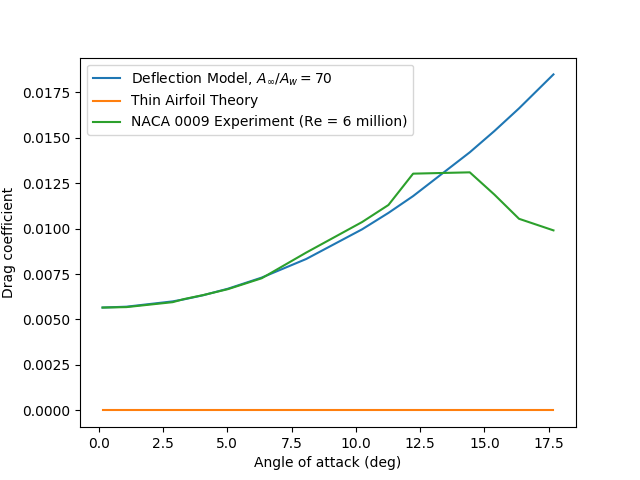
\includegraphics[totalheight=4.5cm]{cd}
\caption{Drag coefficient predictions from Thin Airfoil Theory, the present Deflection Theory, and NACA 0009 experimental data.}
\label{fig:cd}
\end{figure}

\begin{figure}[htb]
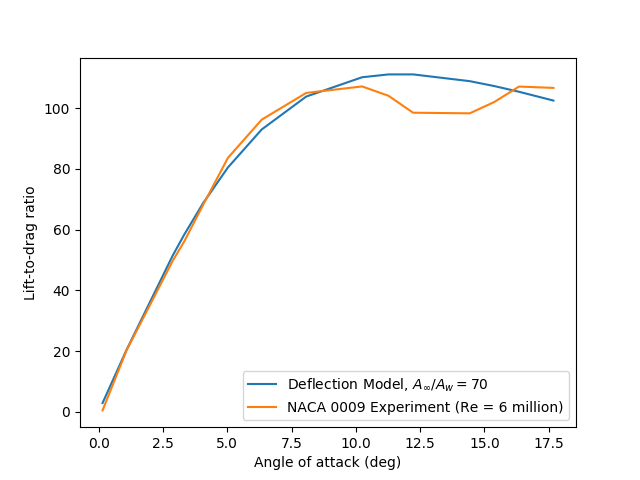
\includegraphics[totalheight=4.5cm]{ld}
\caption{Lift-to-drag ratio predictions from the present Deflection Theory, and NACA 0009 experimental data.}
\label{fig:ld}
\end{figure}

Figures \ref{fig:cl_ratio}, \ref{fig:cd_ratio}, and \ref{fig:ld_ratio} show the sensitivity of performance on \(A_\infty / A_w\).
Lift predictions are much less sensitive to \(A_\infty / A_w\) than the drag predictions are.

\begin{figure}[htb]
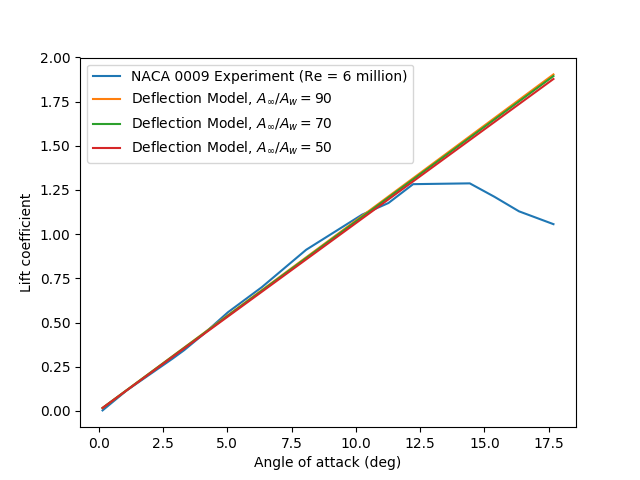
\includegraphics[totalheight=4.5cm]{cl_ratio}
\caption{Sensitivity of Deflection Theory lift predictions to the \(A_\infty / A_w\) parameter.}
\label{fig:cl_ratio}
\end{figure}

\begin{figure}[htb]
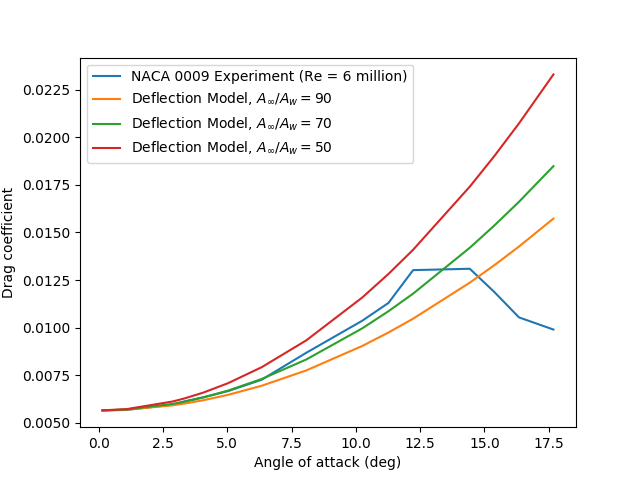
\includegraphics[totalheight=4.5cm]{cd_ratio}
\caption{Sensitivity of Deflection Theory drag predictions to the \(A_\infty / A_w\) parameter.}
\label{fig:cd_ratio}
\end{figure}

\begin{figure}[htb]
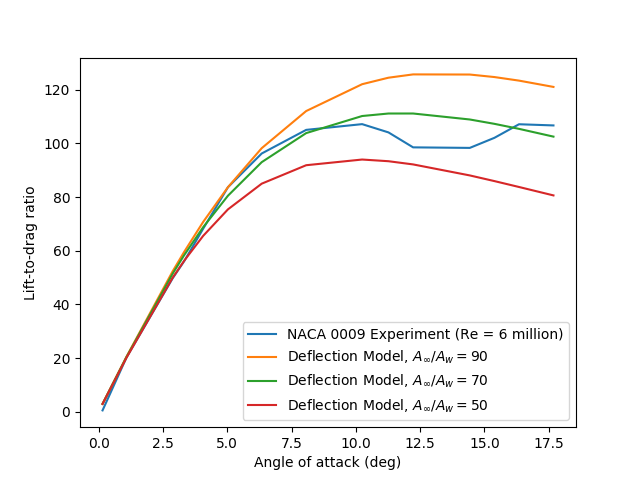
\includegraphics[totalheight=4.5cm]{ld_ratio}
\caption{Sensitivity of Deflection Theory lift-to-drag ratio predictions to the \(A_\infty / A_w\) parameter.}
\label{fig:ld_ratio}
\end{figure}


\section{Discussion}

Deflection Theory is a novel physical argument somewhat corroborated by experimental data and provides a possible way to better understand lift and drag.
It is important to remember that for a complete performance prediction model, Deflection Theory requires another method to compute \(C_N\).
In this paper, Deflection Theory was used to enhance Thin Airfoil Theory.
The same can be easily done for Vortex Panel Methods.

Deflection Theory explains drag produced by unsteady means, including when no net lift is generated.
Freestream deflection oscillation such that the mean lift is zero will result in a non-zero drag.
Similarly, simultaneous steady opposing flow deflections can also produce non-zero drag without net lift.

It was expected for the model derived in this paper to match well with experiment until stall, because Thin Airfoil Theory was used to compute \(C_N\).
A stalled airfoil is not an effective deflector of the freestream flow, but the Deflection Theory still holds.
Computing the \(C_N\) is not the responsibility of Deflection Theory.

Currently the lack of a method to determine the extent of the freestream flow that interacts with the airfoil, represented by the parameter \(A_\infty / A_w\), is the most glaring deficiency.
However, it might be reasonable to empirically determine an estimate for a set of similar airfoils.


%Citation example \cite{Figueredo:2009dg}.


%\begin{thebibliography}{99} % Bibliography - this is intentionally simple in this template

\bibitem[Figueredo and Wolf, 2009]{Figueredo:2009dg}
%Figueredo, A.~J. and Wolf, P. S.~A. (2009).
\newblock Assortative pairing and life history strategy - a cross-cultural
  study.
\newblock {\em Human Nature}, 20:317--330.

\end{thebibliography}


\end{document}
